\documentclass[a4paper,12pt]{article}
\usepackage{amsmath, amsthm, amssymb}
\usepackage{datetime}
\usepackage{framed}
\usepackage{enumitem}
\usepackage{fancyref}
\usepackage{wrapfig}
\usepackage{pifont}

\usepackage{csquotes}
\renewcommand{\mkbegdispquote}[2]{\itshape}

\usepackage{data/circledsteps}
\usepackage[top=1in,bottom=1in,left=1in,right=1in]{geometry} % 用于设置页面布局
\usepackage{xeCJK} % 用于使用本地字体
\usepackage[super, square, sort&compress]{natbib} % 处理参考文献
\usepackage{titlesec, titletoc} % 设置章节标题及页眉页脚
%\usepackage{xCJKnumb} % 中英文数字转换
\usepackage{amssymb}
\usepackage{amsmath} % 在公式中用\text{文本}输入中文
\usepackage{diagbox}
\usepackage{multirow} % 表格中使用多行
\usepackage{booktabs} % 表格中使用\toprule等命令
\usepackage{rotating} % 使用sidewaystable环境旋转表格
\usepackage{tabularx}
\usepackage{graphicx} % 处理图片
\usepackage{footnote} % 增强的脚注功能,可添加表格脚注
\usepackage{threeparttable} % 添加真正的表格脚注,示例见README
\usepackage{hyperref} % 添加pdf书签

\usepackage{tikz}
\usetikzlibrary{shapes,arrows,shadows}

% 字体设置
\setmainfont{Times New Roman}
\setsansfont[Scale=MatchLowercase,Mapping=tex-text]{PT Sans}
\setmonofont[Scale=MatchLowercase]{PT Mono}
\setCJKmainfont[ItalicFont={Kaiti SC}, BoldFont={Heiti SC}]{Songti SC}
\setCJKsansfont{Heiti SC}
\setCJKmonofont{Songti SC}
% \setCJKmainfont[BoldFont={FZXiaoBiaoSong-B05S}]{Songti SC}
% \setCJKfamilyfont{kai}[BoldFont=Heiti SC]{Kaiti SC}
% \setCJKfamilyfont{song}[BoldFont=Heiti SC]{Songti SC}
% \setCJKfamilyfont{hei}[BoldFont=Heiti SC]{Heiti SC}
% \setCJKfamilyfont{fsong}[BoldFont=Heiti SC]{Songti SC}
% \newcommand{\kai}[1]{{\CJKfamily{kai}#1}}
% \newcommand{\hei}[1]{{\CJKfamily{hei}#1}}
% \setromanfont[Mapping=tex-text]{TeXGyrePagella}
% \setsansfont[Scale=MatchLowercase,Mapping=tex-text]{TeXGyrePagella}
% \setmonofont[Scale=MatchLowercase]{Courier New}
%%设置常用中文字号,方便调用
\newcommand{\erhao}{\fontsize{22pt}{\baselineskip}\selectfont}
\newcommand{\xiaoerhao}{\fontsize{18pt}{\baselineskip}\selectfont}
\newcommand{\sanhao}{\fontsize{16pt}{\baselineskip}\selectfont}
\newcommand{\xiaosanhao}{\fontsize{15pt}{\baselineskip}\selectfont}
\newcommand{\sihao}{\fontsize{14pt}{\baselineskip}\selectfont}
\newcommand{\xiaosihao}{\fontsize{12pt}{\baselineskip}\selectfont}
\newcommand{\wuhao}{\fontsize{10.5pt}{\baselineskip}\selectfont}
\newcommand{\xiaowuhao}{\fontsize{9pt}{\baselineskip}\selectfont}
\newcommand{\liuhao}{\fontsize{7.5pt}{\baselineskip}\selectfont}

% 章节标题显示方式及页眉页脚设置
% \item xCJKnumb是自己额外安装的包
% \item titleformat命令定义标题的形式
% \item titlespacing定义标题距左、上、下的距离
\titleformat{\section}{\raggedright\large\bfseries}{\thesection}{1em}{}
\titleformat{\subsection}{\raggedright\normalsize\bfseries}{\thesubsection}{1em}{}
\titlespacing{\section}{0pt}{*0}{*2}
\titlespacing{\subsection}{0pt}{*0}{*1}
% 由于默认的2em缩进不够,所以我手动调整了,但是在windows下似乎2.2就差不多了,或者是article中没有这个问题
\setlength{\parindent}{2.2em}

% 设置表格标题前后间距
\setlength{\abovecaptionskip}{0pt}
\setlength{\belowcaptionskip}{0pt}


\renewcommand{\refname}{\bfseries{参~考~文~献}} %将Reference改为参考文献(用于 article)
% \renewcommand{\bibname}{参~考~文~献} %将bibiography改为参考文献(用于 book)
\renewcommand{\baselinestretch}{1.38} %设置行间距
\renewcommand{\figurename}{\small\ttfamily 图}
\renewcommand{\tablename}{\small\ttfamily 表}


\usepackage{stmaryrd}
\usepackage{mathtools}


\title{再论“自然语言编程”的不智}
\date{2023 年}
\author{苑明理}

\begin{document}

\maketitle{}
\centerline{ 苑明理 }

\centerline{\rule{14cm}{0.4pt}}
\begin{displayquote}
Edsger W. Dijkstra 在 1978 年写下了一篇短述《论“自然语言编程”的不智》,质疑“自然语言编程”会简化工作,指出只有排除了谬误的形式方法才是真正有效率的方法。
本文从历史、实务层面和理论三层面对这一短述展开反思。
\end{displayquote}
\centerline{\rule{13cm}{0.4pt}}
\renewcommand{\contentsname}{\hfill\bfseries 目录\hfill}
\setcounter{tocdepth}{2}
\tableofcontents
\centerline{\rule{13cm}{0.4pt}}
\newpage

1978 年 Edsger W. Dijkstra 在回顾编程语言早期历史时,讨论到当时人们关于“自然语言编程”的观点,他认为这种观点是不明智的,于是写下了一篇很短的论述《论“自然语言编程”的不智》。


\begin{wrapfigure}{r}{0.35\textwidth}
    \centering
    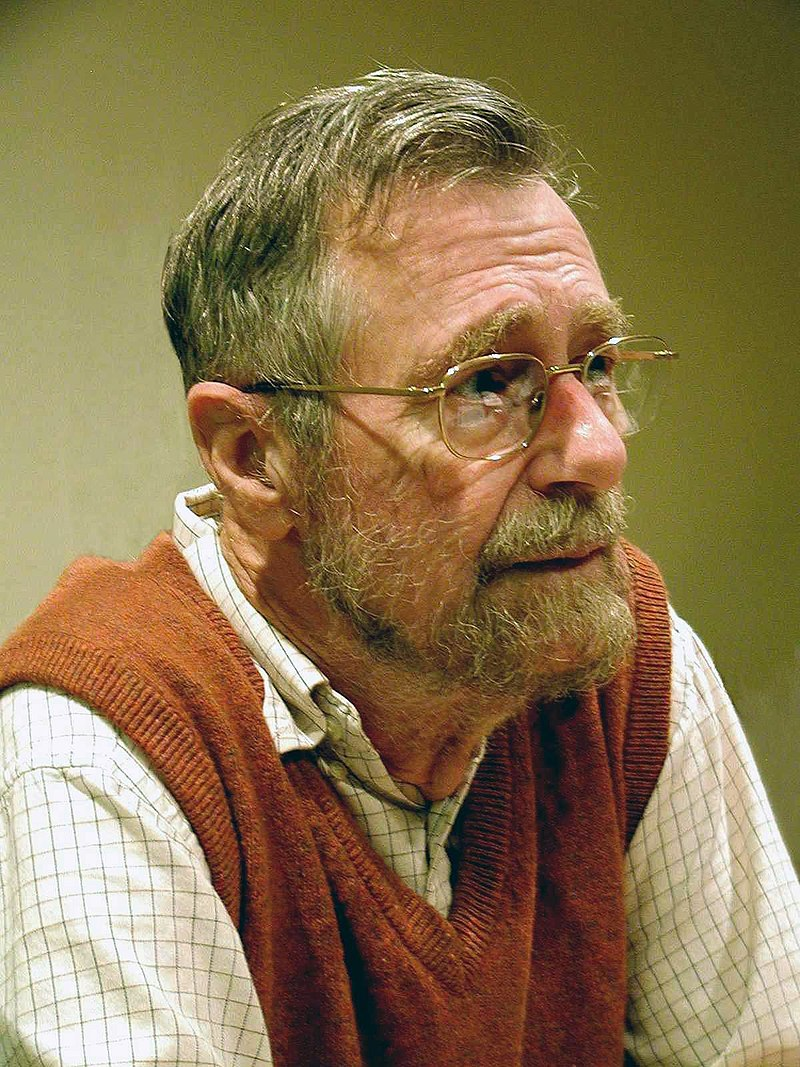
\includegraphics[height=2.0in]{images/Edsger_Wybe_Dijkstra.jpeg}
    \caption{Edsger W. Dijkstra}
\end{wrapfigure}

在 2023 年初 OpenAI 带来的 ChatGPT 才刚刚开始发酵;到了年末,所有的学界与业内的参与者都感受到了大模型的巨大力量。
人们普遍相信各种类型的大模型可以加速行业的运行,而大语言模型(LLM)是其中最受期待的。一方面,LLM 被认为是通向 AGI 最可能的路径;
另一方面,LLM 能够更好地理解人类语言,人们相信它可以把人类智能及机器智能更佳地连接在一起。

上述第二点的落实必然涉及自然语言编程,那么我们应该如何理解 1978 年 Dijkstra 的论述呢?
表面上,Dijkstra 的论点和当今人们的普遍预期是矛盾的,但这个落差背后的意义与可能性仍然值得深入思考。

\section{E. W. Dijkstra 的论点}

Edsger W. Dijkstra 对“自然语言编程”的论点主要来自如下两部分陈述:

他质疑“自然语言编程”会简化工作的想法。

\begin{displayquote}
为了让机器使用更加简便,有人提出了一个想法:(尝试)设计可以接受我们用母语发出的指令的机器。诚然,这会让机器变得更复杂,但有人辩称,通过让机器承担更重的负担,我们的生活将变得更轻松。如果你认为使用形式符号体系是造成困难的根源,这看起来似乎合理。但这个论点真的成立吗?我对此表示怀疑。

我们现在明白,选择一个界面不仅仅是(固定数量的)工作分配问题,因为还必须考虑界面上进行协作和交流所涉及的工作。根据我们的实际经验—我不得不说,这是一种警醒的体验—我们知道,改变界面很容易在界面两侧都增加工作量(有时甚至是极大的增加)。因此,现在更倾向于使用所谓的“狭窄界面”。所以,变成用人类的母语进行机器与人的交流会大幅增加机器的负担,我们还是不得不对这样做会简化人类生活的假设提出质疑。
\end{displayquote}

他继而又强调了来自 Vieta、Descartes、Leibniz 和 Boole 等人的形式方法的学术传统,认为这种排除了谬误的工具,才是真正有效率的。

\begin{displayquote}
形式文本的优点在于,它们的操作要合法,只需遵守一些简单的规则。仔细想想,你会发现它们是一种极其有效的工具,能够排除各种荒谬,这些荒谬在我们使用母语时几乎是不可避免的。

我们不应将使用形式符号看作一种负担,反而应将使用它们的便利视为一种特权:得益于它们,学生们能够学会做过去只有天才才能完成的事情。总而言之,我们使用母语的“自然”实质上就是我们轻易地使用它们来发表那些荒谬的言论的能力。
\end{displayquote}

\section{历史的回顾}

计算作为一种学科范式是在 1930 年代建立起来的。1936 年 Church、Turing和 Kleene 等人相继发表了论文,奠定了计算理论的基础。
1936 年,Alonzo Church 发表了《可计算数的一般性质》(An Unsolvable Problem of Elementary Number Theory),提出了著名的 Church-Turing 假设;1936 年,Alan Turing 发表了《论可计算数及其在判定问题上的应用》(On Computable Numbers, with an Application to the Entscheidungsproblem),提出了著名的图灵机模型;1936 年,Stephen Kleene 发表了《可计算函数的一般性质》(General Recursive Functions of Natural Numbers),提出了著名的递归函数模型。
他们的工作都和 Hilbert 的 Entscheidungsproblem 问题有关系,旨在探讨人类数学能力的边界。其中 Turing 的工作涉及图灵机,是一种机器的隐喻形式。
图灵机的提出,使得计算理论的研究从数学的角度转向了机器的角度,成为计算机科学的起源。Turing 也很早讨论智能的问题,他在 1950 年发表的《计算机器与智能》(Computing Machinery and Intelligence)中提出了著名的图灵测试,认为智能是一种不可定义的概念,只能通过测试来判断。

\begin{figure}[ht]
    \centering
    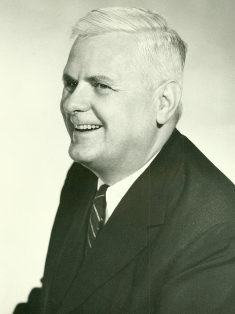
\includegraphics[height=1.5in]{images/alonzo_church.jpg}
    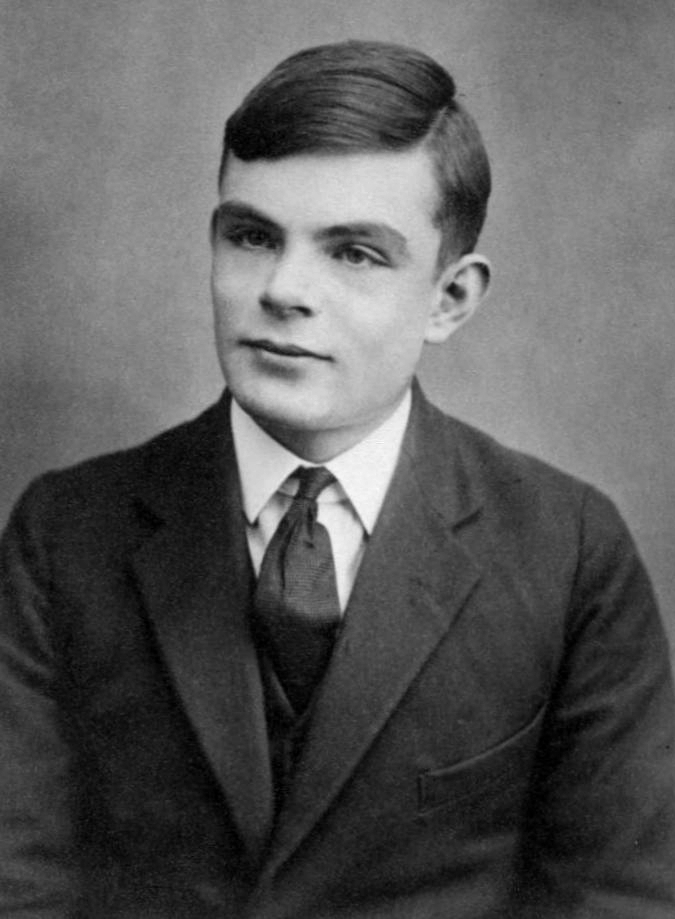
\includegraphics[height=1.5in]{images/alan_turing.jpg}
    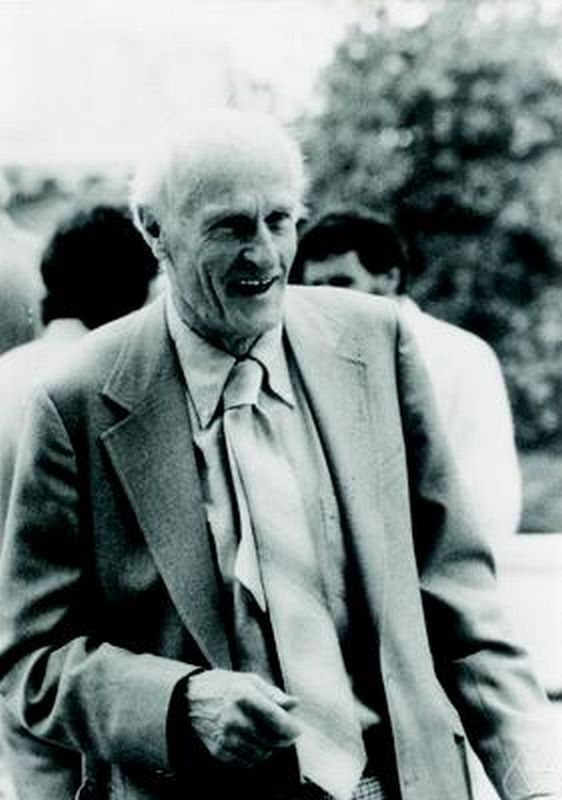
\includegraphics[height=1.5in]{images/kleene.jpg}
    \includegraphics[height=1.5in]{images/emil_post.jpeg}
    \caption{青年图灵}
\end{figure}

\begin{figure}[ht]
    \centering
    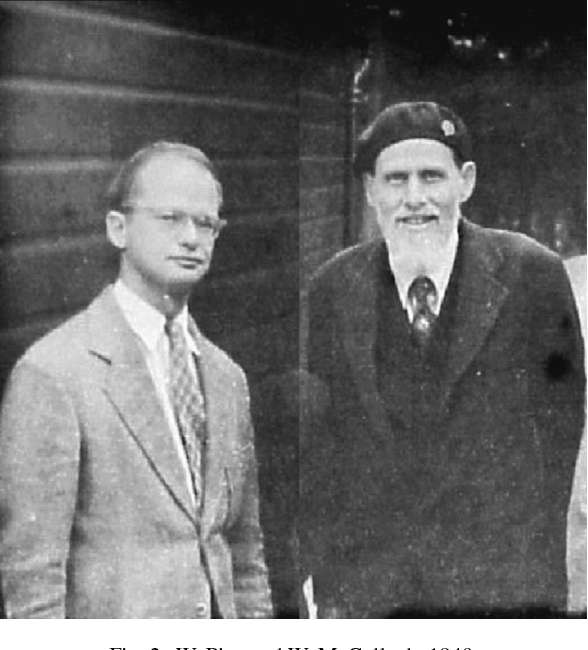
\includegraphics[height=2.0in]{images/pitts_mcculloch_1949.png}
    \caption{Pitts和Mcculloch在 1949 年的合照}
\end{figure}

神经网络

智能

学习

深度学习

语言模型

\section{计算与智能的差异}

让我们看一下 OpenAI 在 2023 年 11 月发布 ChatGPT4 最新版的表现。

\begin{displayquote}
    【提问者】我有二十个随机排列的自然数,每个数都不大于 20,请问我把这二十个数排序之后,结果是什么样的?

    【ChatGPT】你好,你这个问题真是个数学版本的“猜猜我心里想的是什么数字”!既然你给出的数字是随机的,而且我没有具体的数字列表,那我就只能猜了:它们排序后可能是1到20的任何一种排列,或者还可能包含重复的数字,也可能不全。不过,如果你有具体的数字列表,我可以帮你把它们排序哦!
\end{displayquote}



\begin{displayquote}
    【提问者】我有二十个随机排列的彼此不同的自然数,每个数都不大于 20,请问我把这二十个数排序之后,结果是什么样的?

    【ChatGPT】明白了!既然你有二十个彼此不同的自然数,每个数都不大于20,并且要求排序后的结果,那么这些数字肯定是1到20这20个自然数的某种排列。因为只有这20个数字满足你的条件,且它们互不相同。排序后,结果就是从1到20的升序排列。简单来说,就是:

    1, 2, 3, 4, 5, 6, 7, 8, 9, 10, 11, 12, 13, 14, 15, 16, 17, 18, 19, 20

    数学的美妙之处就在于它的确定性和逻辑性,不是吗?
\end{displayquote}

\begin{displayquote}
    【提问者】我有一万个随机排列的彼此不同的自然数,每个数都不大于一万,请问我把这一万个数排序之后,结果是什么样的?

    【ChatGPT】这个问题的答案其实跟之前20个数字的情况类似。既然你有一万个彼此不同的自然数,且每个数都不大于一万,那么这些数字必然是从1到10000的所有自然数。所以,当你对这些数进行排序后,结果将是一个从1到10000的升序排列。简而言之,就是:

    1, 2, 3, 4, 5, 6, 7, 8, 9, 10, ..., 9999, 10000

    这就是数学之美,简单又直接!
\end{displayquote}

\begin{displayquote}
    【提问者】我有二十个随机排列的彼此不同的自然数,每个数都不大于 100,请问我把这二十个数从小到大排序之后,结果是什么样的? 这 20 个数字是  97、25、84、56、77、13、42、66、95、11、62、49、6、57、82、34、78、52、3、29

    【ChatGPT】排序后的20个数从小到大排列如下:

    3, 6, 11, 13, 25, 29, 34, 42, 49, 52, 56, 57, 62, 66, 77, 78, 82, 84, 95, 97

    数学的确是一种既精确又优美的语言!
\end{displayquote}


有了上面的实验和理解,我们确实会对“自然语言编程”拥有一定的信心。但是,我们仍然需要进行更深入的分析。

\section{关于智能的定义}

快速找到问题求解中捷径的能力。

\section{关于编程}

抽象的论述一种还没有充分发展的编程形态是一个困难的事情,让我们尝试举几个例子,通过例子来理解 Dijkstra 的论述和讨论“自然语言编程”的可能性。

\subsubsection{确定性的编程}

\subsubsection{不确定性的编程}

\subsubsection{适应性的编程}

\subsubsection{智能的编程}

\section{复杂适应系统}

模块的思想

\section{确定性与正确性的来源}

\section{语言}

\newpage

\appendix

\section{论“自然语言编程”的不智}

从自动计算的早期开始,总有人认为编程必须如同使用任何形式符号体系那样的精确与谨慎是一种缺陷。他们批评机器对于其执行的指令过于严格的服从性,哪怕稍加思考就能发现这些指令明显错误。正如A.E.Houseman所说:“但一刻钟对于思考来说是很长的时间,而思考本身是个痛苦的过程。” 他们热切地期待并寻找那些更智能的机器,它们能拒绝执行明显愚蠢的任务,如小错误引发的活动。
\footnote{原文位于 E. W. Dijkstra Archive 编号 667 手稿,原题目 \href{https://www.cs.utexas.edu/users/EWD/ewd06xx/EWD667.PDF}{On the foolishness of "natural language programming"};本译文的插图均由译者添加,图片来自维基媒体共享资源网站}

机器代码,由于几乎不包含任何冗余,很快就被认为是人与机器之间不必要的风险界面。部分作为对这种看法的回应,所谓的“高级编程语言”应运而生,随着时间的推移,我们学会了在一定程度上增强了对愚蠢错误的防护。一个重要的进步是,现在许多愚蠢的错误将导致错误信息的产生,而不是错误的结果。(甚至这种改进并不是普遍受欢迎:有些人发现无法忽略的错误信息比错误的结果更令人烦恼,而在评价编程语言的相对优势时,一些人仍然倾向于将“编程的简易度”与犯下未被察觉错误的容易度相等同。)然而,与编程语言相对应的(抽象)机器仍然是一个忠实的奴隶,即那种完全能够执行无意义指令的非理性自动机。编程仍然是使用形式化的符号体系,因此,依旧需要之前所要求的那种精确和谨慎。

\begin{figure}[ht]
\centering
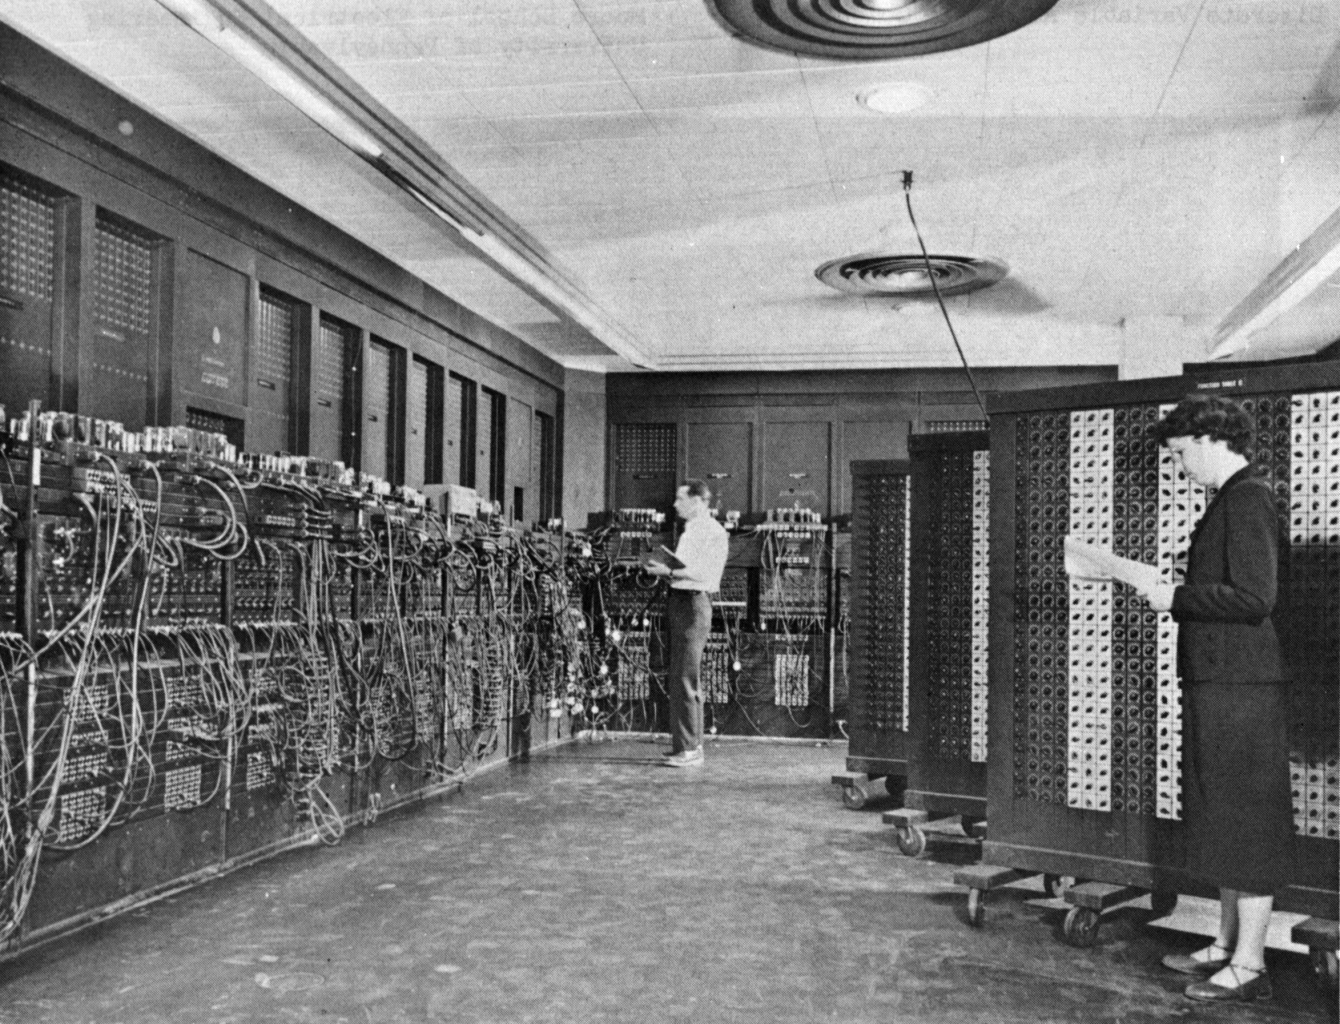
\includegraphics[height=2.5in]{images/ENIAC.jpeg}
\caption{世界上第一台计算机 ENIAC}
\end{figure}

为了让机器使用更加简便,有人提出了一个想法:(尝试)设计可以接受我们用母语发出的指令的机器。诚然,这会让机器变得更复杂,但有人辩称,通过让机器承担更重的负担,我们的生活将变得更轻松。如果你认为使用形式符号体系是造成困难的根源,这看起来似乎合理。但这个论点真的成立吗?我对此表示怀疑。

我们现在明白,选择一个界面不仅仅是(固定数量的)工作分配问题,因为还必须考虑界面上进行协作和交流所涉及的工作。根据我们的实际经验—我不得不说,这是一种警醒的体验—我们知道,改变界面很容易在界面两侧都增加工作量(有时甚至是极大的增加)。因此,现在更倾向于使用所谓的“狭窄界面”。所以,变成用人类的母语进行机器与人的交流会大幅增加机器的负担,我们还是不得不对这样做会简化人类生活的假设提出质疑。

\begin{figure}[ht]
\centering
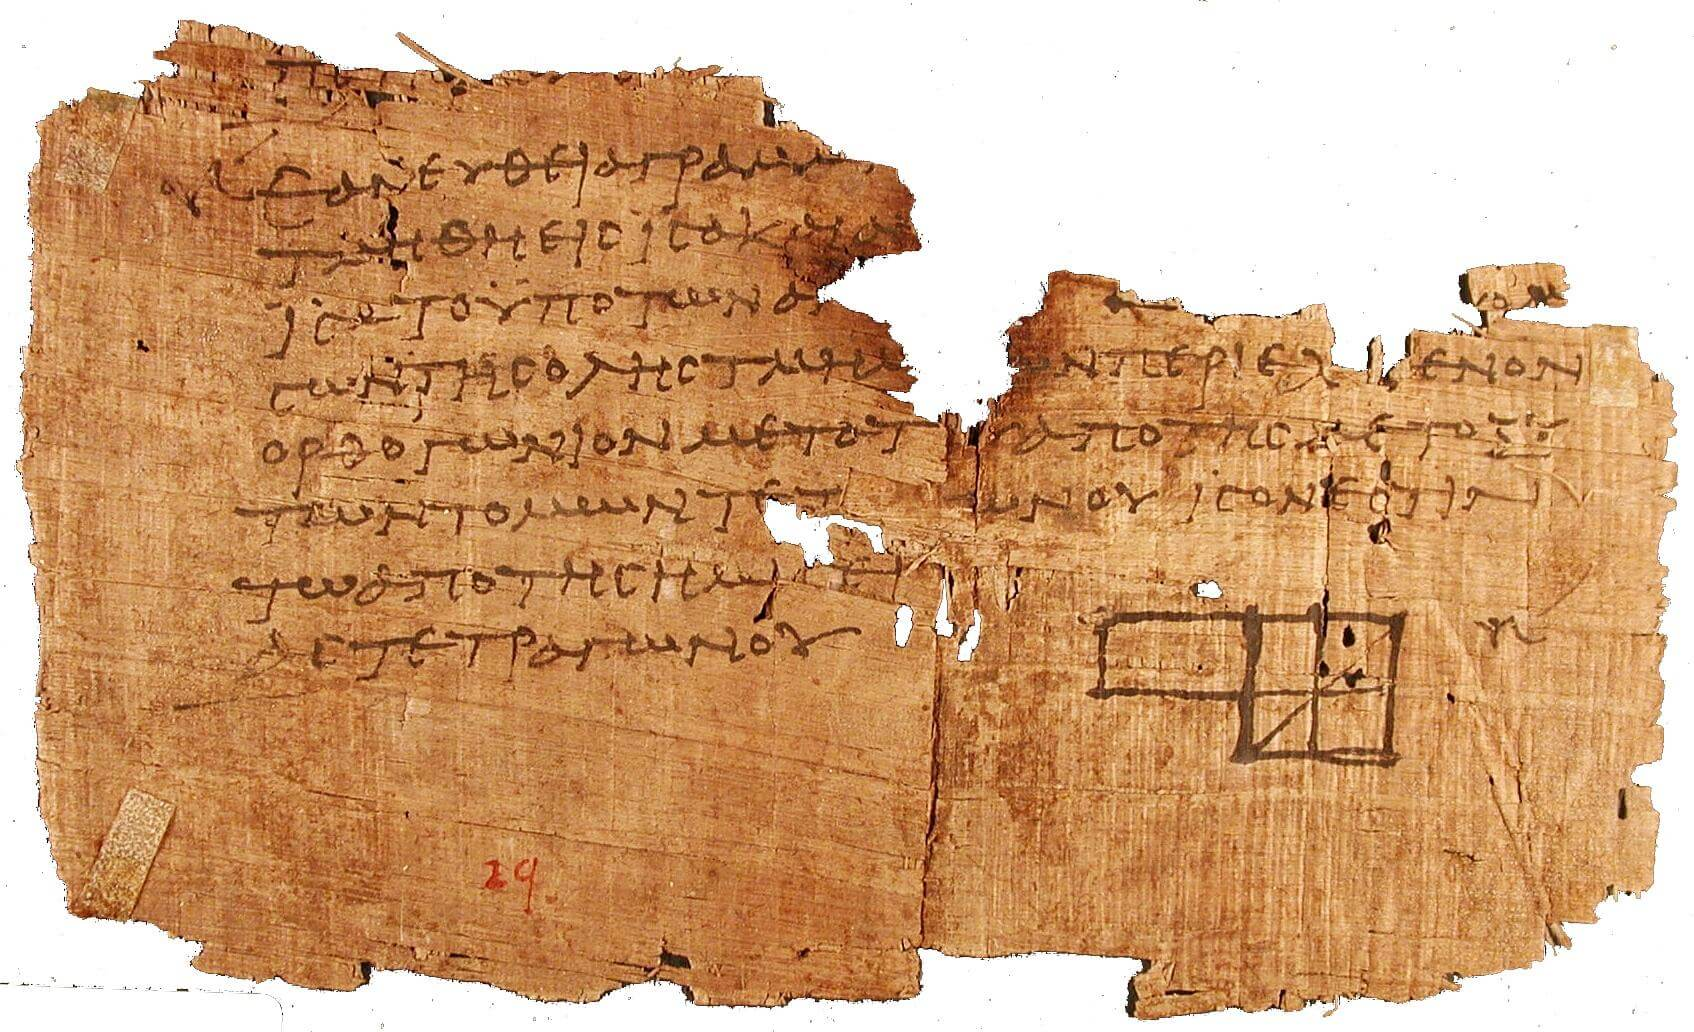
\includegraphics[height=2.0in]{images/elements.jpeg}
\caption{《几何原本》残片}
\end{figure}

简单回顾数学史就能证明这种挑战有多么有道理。希腊数学之所以停滞不前,是因为它一直停留在口头和图像化的层面上;穆斯林的“代数”在尝试使用符号之后变得胆怯,当它回归修辞风格时便走向了衰亡。现代文明世界能够出现—无论是好是坏—是因为西欧能够摆脱中世纪经院哲学的枷锁—那是对语言精确性的徒劳尝试!—这要归功于像 Vieta、Descartes、Leibniz 和(后来的)Boole等人精心设计或至少是有意识设计的形式符号。

\begin{figure}[ht]
\centering
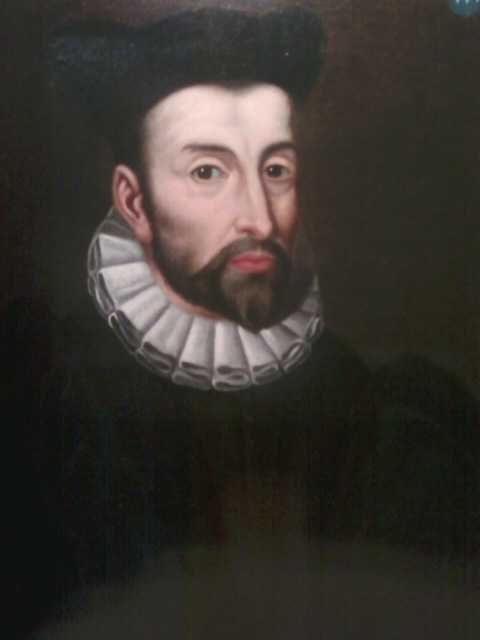
\includegraphics[height=1.5in]{images/Francois_Viete.jpeg}
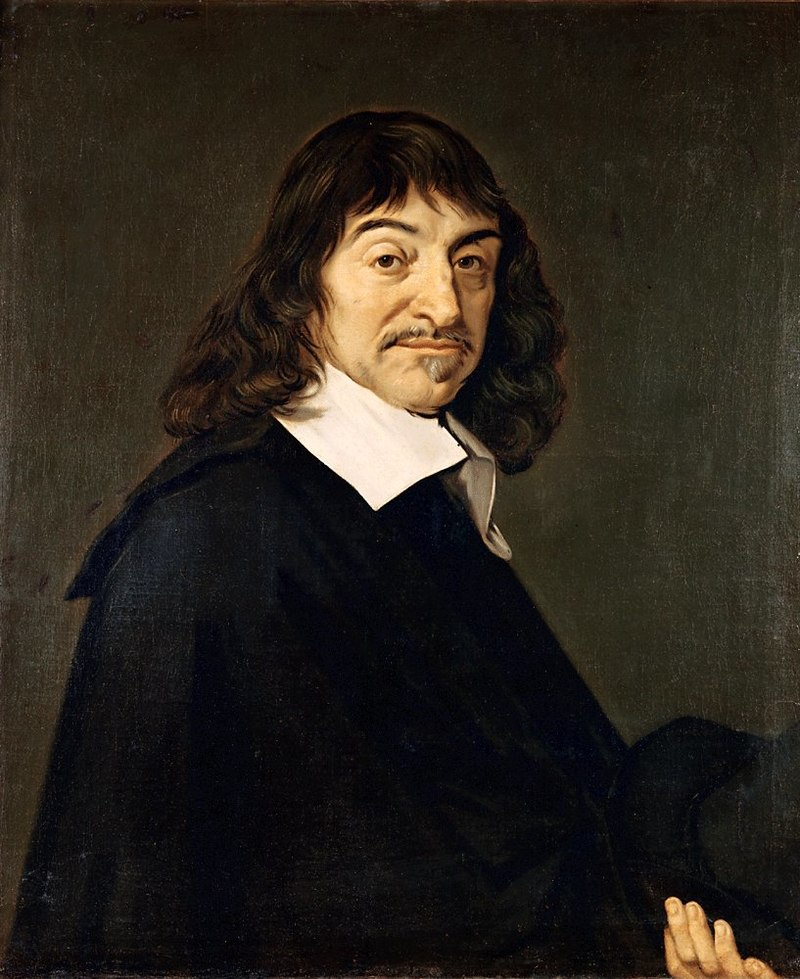
\includegraphics[height=1.5in]{images/Descartes.jpeg}
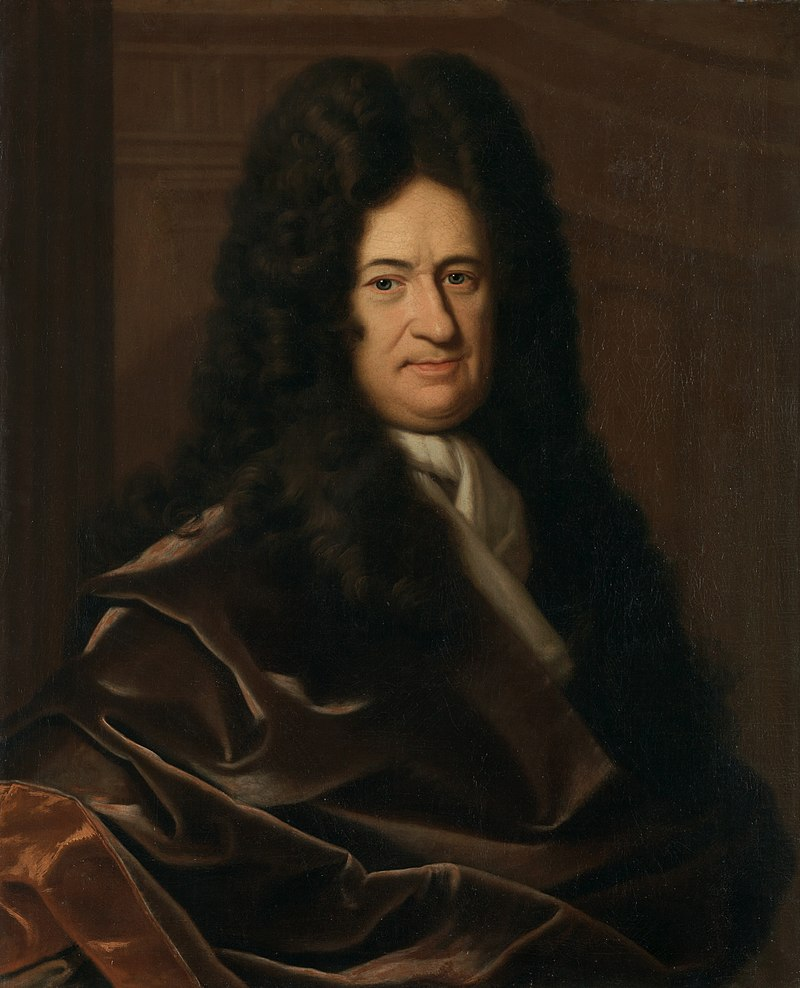
\includegraphics[height=1.5in]{images/Leibniz.jpeg}
\caption{Vieta、Descartes、Leibniz 像}
\end{figure}

形式文本的优点在于,它们的操作要合法,只需遵守一些简单的规则。仔细想想,你会发现它们是一种极其有效的工具,能够排除各种荒谬,这些荒谬在我们使用母语时几乎是不可避免的。

\begin{figure}[ht]
\centering
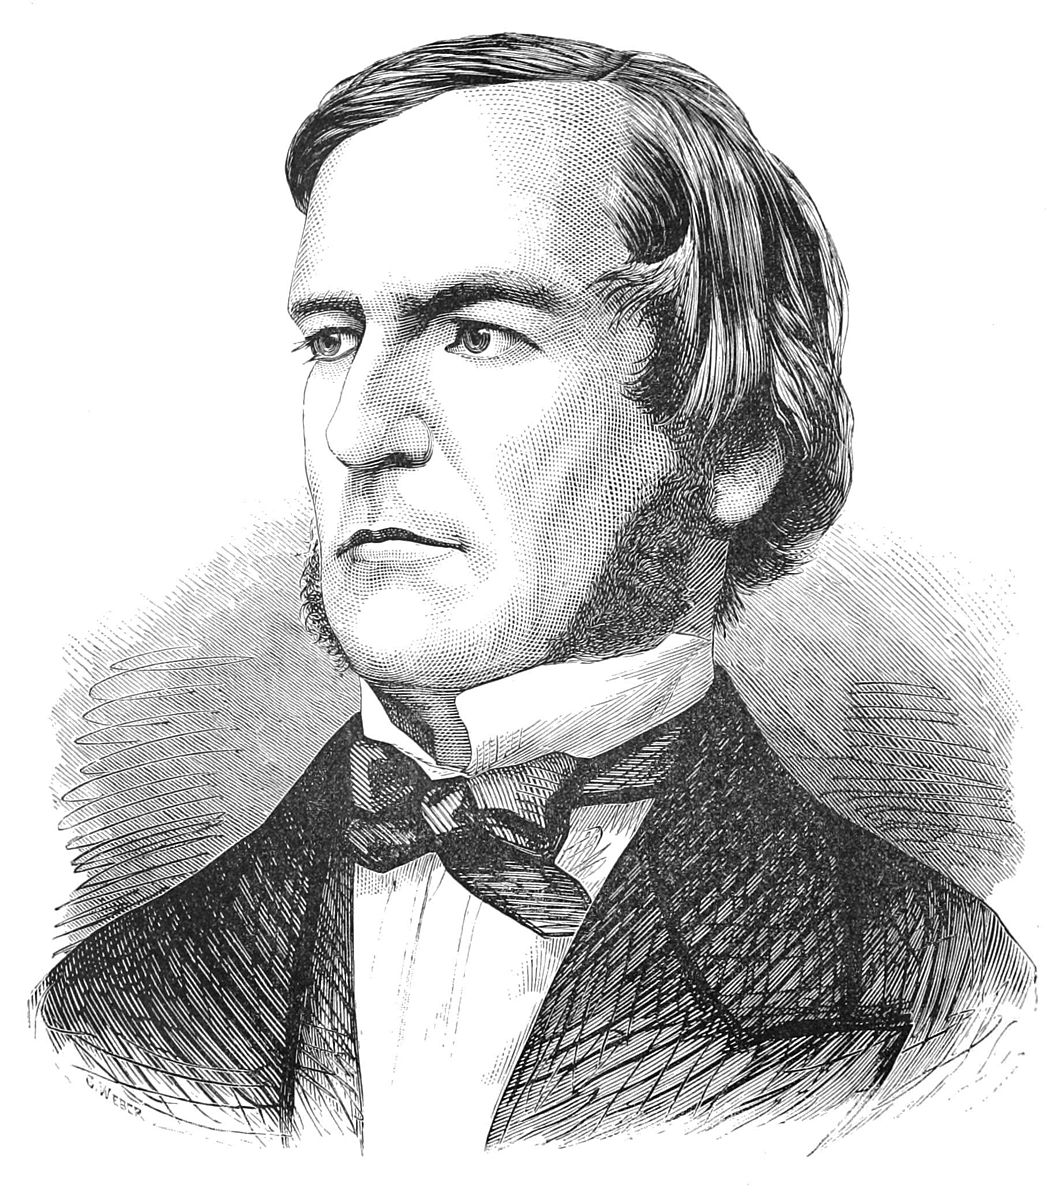
\includegraphics[height=2.0in]{images/George_Boole.jpeg}
\caption{George Boole 像}
\end{figure}

我们不应将使用形式符号看作一种负担,反而应将使用它们的便利视为一种特权:得益于它们,学生们能够学会做过去只有天才才能完成的事情。(显然,这点并没有被1977年在一份技术报告前言中写到的作者理解,他甚至为了所谓的“清晰”,避免使用逻辑连接符的标准符号。这句话的出现表明,这种误解并不仅限于他一人。)总而言之,我们使用母语的“自然”实质上就是我们轻易地使用它们来发表那些荒谬的言论的能力。
\footnote{【原作者按】由于教育趋势偏离了智力训练,过去几十年来,在西方世界,人们对自己语言的掌握程度显著下降:许多按上一代标准来看应该更懂得的人,现在已经无法有效使用自己的母语,即使是在它相当适用的情况下也是如此。(你只需要看看科学文章、技术报告、政府出版物等中那些令人担忧的、在仔细阅读后显得毫无意义的冗长文字。)这一现象—被称为“新文盲”—应当让那些缺乏足够技术洞察力来预测其失败的自然语言编程的信徒们感到泄气。}

尝试想象一下,如果从一开始我们的母语就成为我们信息处理设备的唯一输入和输出方式,可能会有一些启发。我经过深思熟虑的猜想是,历史在某种意义上可能会重演,计算机科学主要将是一种确实深奥的艺术,即如何从那里引导出一个定义足够明确的形式系统。我们将需要动用全世界的智力来使界面足够窄,从而使其可用,并且考虑到人类的历史,猜测要做到足够好可能还需要几千年的时间,这并不是过于悲观的想法。

我从一种强烈的直觉中获得了许多安慰:我怀疑,无论是用荷兰语、英语、美式英语、法语、德语还是斯瓦希里语来编程的机器,它们的制造难度和使用难度都同样巨大。

 \\Plataanstraat 5\\
5671 AL NUENEN\\
荷兰 Edsger W.Dijkstra 教授博士\\
Burroughs 研究员\\

\newpage

\section{Edsger W. Dijkstra 小传}

Edsger W. Dijkstra,1930年5月11日出生于荷兰,是一位杰出的计算机科学家。他在 Amsterdam 大学学习物理和数学,后专注于计算机科学。Dijkstra 的职业生涯始于荷兰的数学中心,并在包括Eindhoven技术大学和美国Texas大学Austin分校等多所大学任教。他因其在编程方法论、操作系统、并发程序设计方面的研究而闻名。

\begin{figure}[ht]
\centering
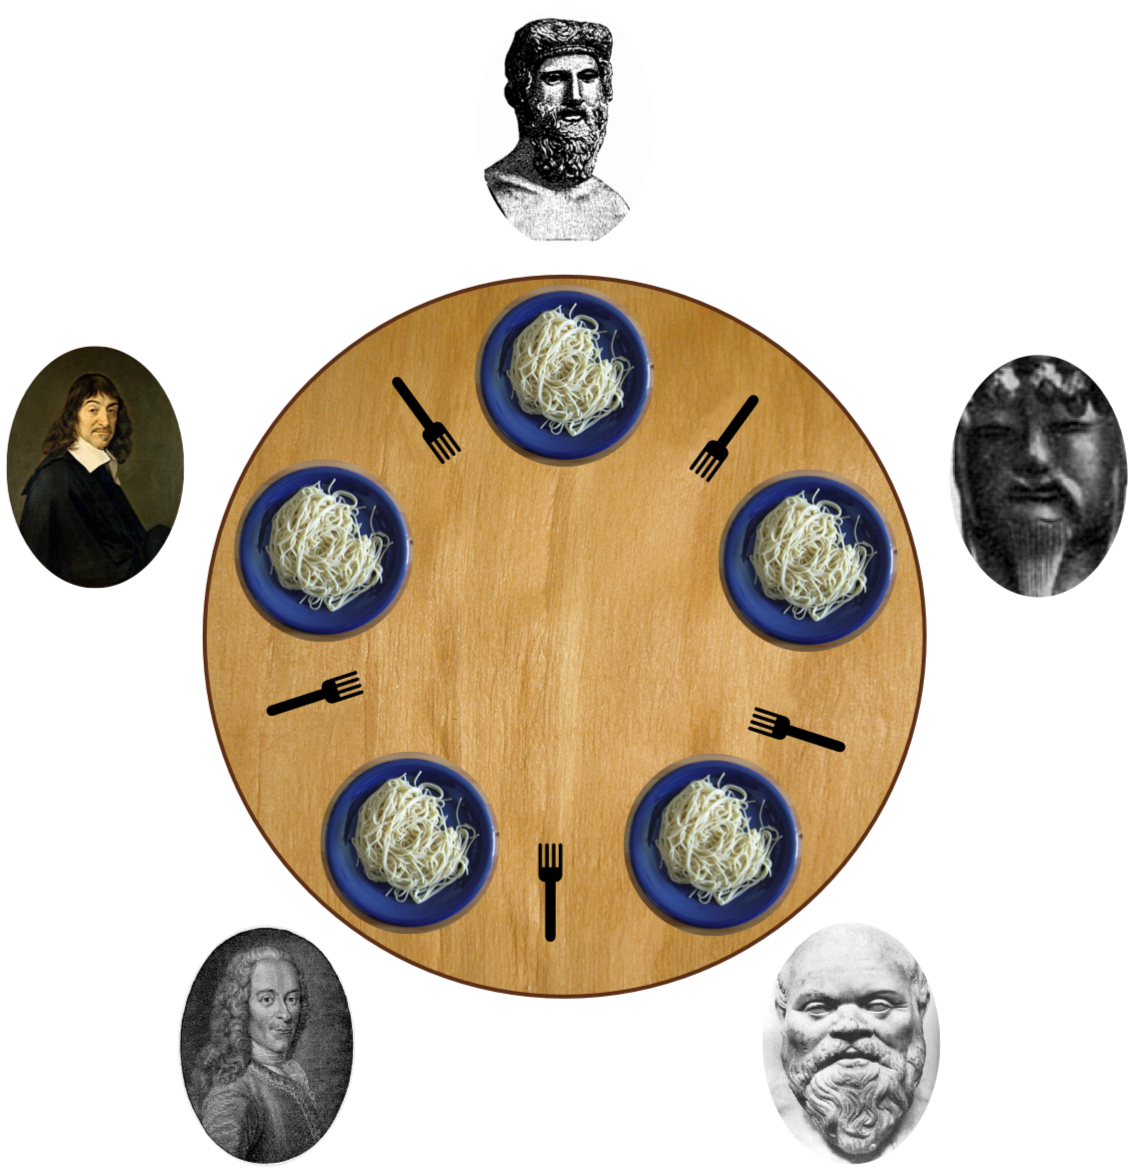
\includegraphics[height=2.5in]{images/dining_philosophers.png}
\caption{由 Dijkstra 提出的哲学家晚餐问题}
\end{figure}

Dijkstra 的主要成就包括创造著名的短路径算法,该算法在网络路由和地图服务中被广泛应用。他是结构化编程的坚定支持者,反对使用GOTO语句,这一观念对现代编程实践和教育产生了重大影响。在操作系统领域,Dijkstra 引入信号量的概念,对进程同步和死锁预防做出了突出贡献。此外,他提出了Communicating Sequential Processes(CSP)模型,极大地推动了并发编程理论和实践的发展。

Dijkstra 还开创了程序的形式方法领域,强调使用数学和逻辑方法表达和验证程序的正确性。这些方法对软件工程至关重要,尤其是在高可靠性和安全关键系统的设计中。

他的成就获得了广泛认可,包括1972年获得的图灵奖。Dijkstra 的工作不仅在他所处的时代具有划时代的意义,而且在当今计算机科学和软件工程领域仍具有深远的影响。2002年8月6日,Dijkstra 在荷兰逝世,但他的理念和研究仍然影响着计算机科学的发展方向。



\end{document}


